% Do not copy directly. Make sure all the sentences are on your own words and properly cite.
\documentclass[12pt]{article}
%\usepackage[round]{natbib} %reference
\usepackage{latexsym,epsfig,graphicx,epstopdf,amsmath,amssymb,amscd,multirow,psfrag,paralist,setspace,dsfont,float}
\usepackage{siunitx} %alignment by decimal
\usepackage[round]{natbib}
\usepackage{upgreek}
\def\baselinestretch{2}
\raggedbottom
\setlength{\abovedisplayshortskip}{1pt}
\setlength{\belowdisplayshortskip}{1pt}
\begin{document}
\title{A Change-Point Detection and Clustering Method in the Recurrent-Event Context}
\author{Qing Li, Kehui Yao, Xinyu Zhang}
\date{}
\maketitle
\newpage
\mbox{} \vspace*{2in}
\begin{center}
\textbf{Author's Footnote:}
\end{center}
Qing Li is an assistant professor in the Department of Industrial \& Manufacturing Systems Engineering, Iowa State University, 3025 Black Engineering Building, Ames, IA 50011.(email: qinglijane@gmail.com), Kehui Yao,Xinyu Zhang.




\newpage

\begin{center}
\textbf{Abstract}

\end{center}
One sentence about the data. A change-point model is usually a natural fit for the time to event data. We can always capture differnet patterns in the clustered data


Recurrent event data has been an interesting topic applied in many fields. When the data is assumed to have one or more clustered subgroups,with each sharing an an unknown change point, we model the data in each subgroup as a non-homogeneous Poisson process with piecewise constant intensity functions. The paper proposes a heurastic clustering method, which divide the data into several clusters based on their similarities defined in a change-point likelihood based model. The method also gives the estimate of the change points, as well as the intensity rates before and after the change point by clusters. It uses the updating scheme motivated by K-means algorithm, but advances the arrangement procedure to be model based, which fits nicely for clustering the recurrent events. The paper also propose a heurastic seraching method to determine the number of underlying clusters, which remains a challenging part for the original K-means problem. Applied into different settings of simulation, the algorithm achieves good performace and is verified to be robust on selecting the appropriate number of clusters. 
%%%%%%%%%%%%%%%%%%%%%%%%%%%%%%%%%%%%%%%%%%%%%%%%%%%%%%%%%%%%%%%%%%%%%%%%

\vspace*{.3in}

\noindent KEY WORDS: {Non-Homogeneous Poisson Process, Recurrent Event, Cluster.}

Note: Supplementary materials for this article are available online.
%%%%%%%%%%%%%%%%%%%%%%%%%%%%%%%%%%%%%%%%%%%%%%%%%%%%%%%%%%%%%%%%%%%%%%%%%%%%%%%%%%%
%%%%%%%%%%%%%%%%%%%%%%%%%%%%%%%%%%%%%%%%%%%%%%%%%%%%%%%%%%%%%%%%%%%%%%%%%%%%%%%%%%%
\section{Introduction}

Recurrent-event data analysis is widely used in various fields such as reliability, medicine, social science and criminology, where a subject or sampling unit has multiple events. 

An interesting problem in recurrent-event data analysis is change-point detection. For example, the events rates of drivers might change as they have more experience and learn from driving education programs; the rate of the recurrent disease episodes may change because of treatment or the effects of the treatment wearing out; the rate of machine malfunction changes because of ageing; the rate of a human behaviour is changing because of certain factors. Detecting the change-point provides critical information on the recurrence patterns, and provide reference for research like what factors caused the change, similarities and heterogeneity among subjects.  

Most of the literatures on change-point detection in recurrent-event context assumed that the event counts follow a non-homogeneous Poisson process (NHPP). The NHPP is a Poisson process whose intensity function is not a constant over time \citep[p.~32]{Ross2006}. Examples include  detecting the change-points in the ozone level by Bayesian method \citep{Cruz2016}, proposing semi-parametric estimators for the change-point when there are multiple individuals \citep{Frobish2016}. 

NHPP with piecewise-constant intensity functions are widely used for change-point detection in the recurrent-event context. For example, \citet{Raftery1986,West1997, Aschar2007, Gupta2015, Montoya2017} developed Bayesian methods to detect the change-points and conducted model selection on the number of change-points for one sampling unit;  \citet{Frobish2009,Li2017b} proposed maximum likelihood estimators (MLE) of change-points for multiple subjects. 

In recurrent-event change-point analysis, clustering the sampling unit is necessary when subgroups exist. Research in this area is limited. \citet{Li2017a} detected the change-points and clustered the individuals using a Bayesian finite mixture model. Such type of methods are relatively complex and computationally expensive.

We assume that there are multiple individuals or sampling units. The recurrent events follow NHPP with piecewise-constant intensity rates. Clusters exist among the individuals. The individuals in the same cluster share the same change-point and the intensity rates. The goal of this paper is to provide an alternative machine learning method to incorporate clustering in recurrent-event change-point analysis.

Notice that clustering is partitioning a set of objects in such a way that objects in the same cluster are more similar to each other, the appropriate clustering algorithm needs to define a distance function to measure the similarity between each object, then minimizing the pairwise distance in the same cluster. For example, when given a set of $m$ data points $D=\left\lbrace x_1,...,x_m\right\rbrace $ in $R^{d}$ and an integer $K$, a heurastic clustering algorithm, K-means, will determine a set of K centroids $C=\left\lbrace c_1,...,c_k\right\rbrace $ in $R^{d}$ so as to minimize the following error function: $E(C)=\Sigma_{x_{\upepsilon D}}min_{k=1,...K}\parallel x-c_k \parallel^{2}$. Even though there exists a wide variety of clustering methods, very few of them can be applied on recurrent events clustering problem because it's hard to find the distance function. The sample unit in this problem is a vector of event times, with arbitrary length, so it cannot be considered as the coordinates in the Euclidean space as the original K-means do. We advance the K-means method by defining the distance function using the probability density function after assuming the sample unit is from some specific distribution.

One advantage for our algorithm is that it can cluster the sample units into different subgroups, as well as give the estimate of change-point and intensity rates before and after the change-point for every subgroups. Another advantage is that it can automatically determine how many clusters the data possesses. Since the original K-means algorithm ofen uses the elbow plot \cite{ketchen1996application} of the within-cluster sum of squares to determine the appropriate number of clusters, the elbow criterion cannot always be unambiguously identified. Our method uses a heurastic searching method, based on the NHPP model, gives a more quantified and reasonable estimate of clusters' numbers. So generally, applying this algorithm on a recurrent events dataset gives us direct knowledge about how many potential similar patterns in the data.


(ADD verifying part with real data)

The algorithm can be divided into four stages. \\
(1) Defining the distance function between the sample units .\\
(2) Cluster the data into a given number of clusters.\\
(3) Introduces two methods of automatically determine the number of clusters. \\
(4) Real data analysis based on the algorithm.


In Section~\ref{sec:models.kmean}, we develop a machine learning method to detect the change-points and cluster the individuals in the recurrent-event context. Simulation study is in Section~\ref{sec:simulation}. A real data analysis is provided in Section~\ref{sec:results}. Section~\ref{sec:discussion} is the conclusion and discussion. %

\section{A Machine Learning Method for Change-Point Detection and Clustering in the Recurrent-Event Context}\label{sec:models.kmean}
% parameters
This section presents a method which combines the K-means clustering algorithm and the likelihood-based change-point detection method in the recurrent-event context in \citet{Frobish2009}. Assume that there are $m$ individuals from $K$ groups with recurrent events, and each individual has an unknown change-point. The individuals in the same cluster share identical change-point and intensity rates. We first show how to estimate the change-point and intensity rates for each cluster.  Then we propose how to cluster the data given the number of groups $K$. Thirdly we show how to automatically detect the number of clusters by a heurastic searching method.


Denote $n_j$ to be the total number of events and $c_j$ be the total follow up time for the $j^{th}$ individual, $j=1,2,\cdots,m$. $c_j$ will be used as the censoring time in the analysis. The events occurred at ordered times $t_{j1},...,t_{jn_j}$.  We assume the $m$ individuals fall in $K$ groups, and the group index is $k$, $k=1,...K$. If an individual $j$ is from group $k$, we denote it as $j \in G_k$. The event counts in group $k$ follow a NHPP with piecewise-constant intensity function $\lambda_k(t)=\lambda_{kb}I(0 \leq t < \tau_k)+\lambda_{ka}I( t\geq \tau_k)$, where $\tau_k$ is the unknown change-point for the $k^{th}$ group and $\tau_k \leq minimum(c_j)$ for $j\in G_k$. $\lambda_{kb}$ is the intensity rate before $\tau_k$, and $\lambda_{ka} $ is the intensity rate after $\tau_k$. Integrating it yields the cumulative intensity function $\Lambda_k(t)=\lambda_{kb}tI(0\leq t<\tau_k)+\left[ \lambda_{kb}\tau_k+\lambda_{ka}(t-\tau_k)\right] I(t\geq \tau_k)$, where $I(t)$ is the indicator function. Let $n_j^{(b)} $ be the number of events for the $j^{th}$ individual before the change-point, and $n_j^{(a)} $ be the number of events after the change-point. Then $n_j^{(b)}+n_j^{(a)}=n_j$. Table \ref{tab:setadd1} gives a summary of the notations. 

\begin{table} [htp]
  %\vspace{-30pt}
   \caption{\label{tab:setadd1} Notations in this paper.}
     \vspace{1ex}
  \centering
  %\hskip-93.5cm
  \begin{tabular}{ll}\hline
      Symbol& Meaning \\\hline
      $m$       & The total number of individuals \\
      $K$       & The total number of groups \\
      $j$       & The individual index, $j=1,2,\cdots,m$ \\
      $n_j$     & The total number of events for the $j^{th}$ individual\\
      $i$       & The event index, $i = 0, 1, 2, \cdots,n_j$, where $i = 0$ indicates the starting point\\
      $t_{ji}$  & The $i^{th}$ event time for the $j^{th}$ individual, assuming $t_{ji_1}\not=t_{ji_2}$ for $\forall j_1\not=j_2$   \\
      $x_{ji}$  & The inter-event time: $x_{ji} = t_{ji} - t_{j,(i-1)}$ \\
    $c_j$     & The follow up time for the $j^{th}$ individual\\
      $k$       & The group index, $k=1,2,\cdots,K$\\
    $N_k$     & The number of individuals in the $k^{th}$ group\\
    $n_j^{(b)}$ & The total number of events for the $j^{th}$ individual before the change-point\\
    $n_j^{(a)}$ & The total number of events for the $j^{th}$ individual after the change-point\\
       $\tau_k$  & The change-point for the $k^{th}$ group\\
      $\lambda_{kb}$& The intensity rate before the change-point for the $k^{th}$ cluster \\
      $\lambda_{ka}$& The intensity rate after the change-point for the $k^{th}$ cluster \\
      \hline
 \end{tabular}%
  \end{table}%
\subsection {Change-point detection by maximizing the likelihood}\label{sec:MLE}
We assume that all the individuals in the same cluster share the identical intensity rates and change-point. Here we summarize the MLEs for $\tau_k,\lambda_{kb}$ and $\lambda_{ka}$ proposed by \citet{Frobish2009}.

 The likelihood for one individual $j$ given that $j \in G_k$ is \citep{Thompson2012}: 
$$L_{j}(\tau_k,\lambda_{kb},\lambda_{ka}|\pmb X_j)=exp[-\Lambda(c_j)]\prod_{i=1}^{n_j}\lambda_j(t_{ji})=exp[-\Lambda(c_j)]\lambda_{kb}^{n_j^{(b)}}\lambda_{ka}^{n_j^{(a)}},$$ where $\pmb X_j = (t_{j1}, \cdots, t_{jn_j}, c_j)^T$.
Denoting $\pmb X_{(k)}$ to be the event times and censoring times in group $k$, the log likelihood of $N_k$ individuals in this group combined is
\begin{equation}
logL_{(k)}(\tau_k,\lambda_{kb},\lambda_{ka}|\pmb X_{(k)})=-(\lambda_{bk}-\lambda_{ak})N_k\tau_k-\lambda_{ak}\sum_{j \in G_k}c_j+\left( \sum_{j \in G_k}n_j^{(b)}\right) log \lambda_{kb}
+\left( \sum_{j \in G_k}n_j^{(a)}\right) log\lambda_{ka}.
\end{equation}

Taking the derivative of $logL_{(k)}$ and setting it to zero,  we can obtain the MLEs for the intensity rates: 
\begin{equation}\label{eqn:lam_MLE}
\hat{\lambda}_{kb}=\frac{\sum_{j \in G_k}n_j^{(b)}}{\tau_kN_k},\hat{\lambda}_{ka}=\frac{\sum_{j \in G_k}n_j^{(a)}}{\sum_{j \in G_k}c_j- \tau_kN_k}.
\end{equation}
The MLEs of the intensity rates are the average number of events per individual per unit time. 

According to \citet{Frobish2009}, the value of $\tau_k$ that maximize $logL_(k)(\tau_k,\hat\lambda_{kb},\hat\lambda_{ka}|\pmb X_{(k)})$ locate at one of the event times, and the MLE of $\tau_k$ is consistent. Therefore, the MLE of $\tau_k$ is the event-time that maximize the log likelihood:  
\begin{equation}\label{eqn:tau_MLE}
\hat\tau_k= argmax_{\tau_k = t_{ji}|j \in G_k, 1\leq i \leq n_j}logL_{(k)}(\tau_k,\hat\lambda_{kb},\hat\lambda_{ka}|\pmb X_{(k)}).
\end{equation} 
Plugqging $\hat\tau_k$ in Eq. \ref{eqn:lam_MLE}, we get the MLEs for the intensity rates $\lambda_{kb},\lambda_{ka}$.
\begin{equation}\label{eqn:lam}
\hat{\lambda}_{kb}=\frac{\sum_{j \in G_k}n_j^{(b)}}{\hat{tau_k}N_k},\hat{\lambda}_{ka}=\frac{\sum_{j \in G_k}n_j^{(a)}}{\sum_{j \in G_k}c_j- \hat{\tau_k}N_k}.
\end{equation}
\subsection{RKmeans clustering}\label{sec:kmean}
We propose a method to cluster the $m$ individuals into $K$ groups given the number of clusters in this section. 

The challenge is that our observation unit $j,~j=1,...,m$ is a sequence of event times, which is high-dimensional data. A natural way to see whether there is heterogeneity among the $m$ individuals is to plot the sequence events of each individual against time. To illustrate this, suppose we have an observation $\pmb X_j = (t_{j1}, \cdots, t_{jn_j}, c_j)$ , which is time-to-event data, where $t_{ji}$ means the $i^{th}$ event time for the $j^{th}$ individual. Denote $n_j^{(i)}$ be total number of events before $t_{ji}$, plot $(t_{ji},n_j^{(i)}),i=1,...,n_j$, which is the function of cumulative event occurences during the time interval $(0,c_j)$.. Suppose 40 individuals are generated from two groups, if we define $(\lambda_{kb},\lambda_{ka},\tau_k)$ as the centroids of group $k$, then the 40 individuals are generated from two groups with centroids $(250,100,300)$ and $(250,100,150)$ respectively. Forty lines are drawn in Fig. \ref{fig:forty_lines} , each represent a sequence of recurrent events. From the plot, we may think that these individuals can be divided into two groups.





\begin{figure} [htp]
 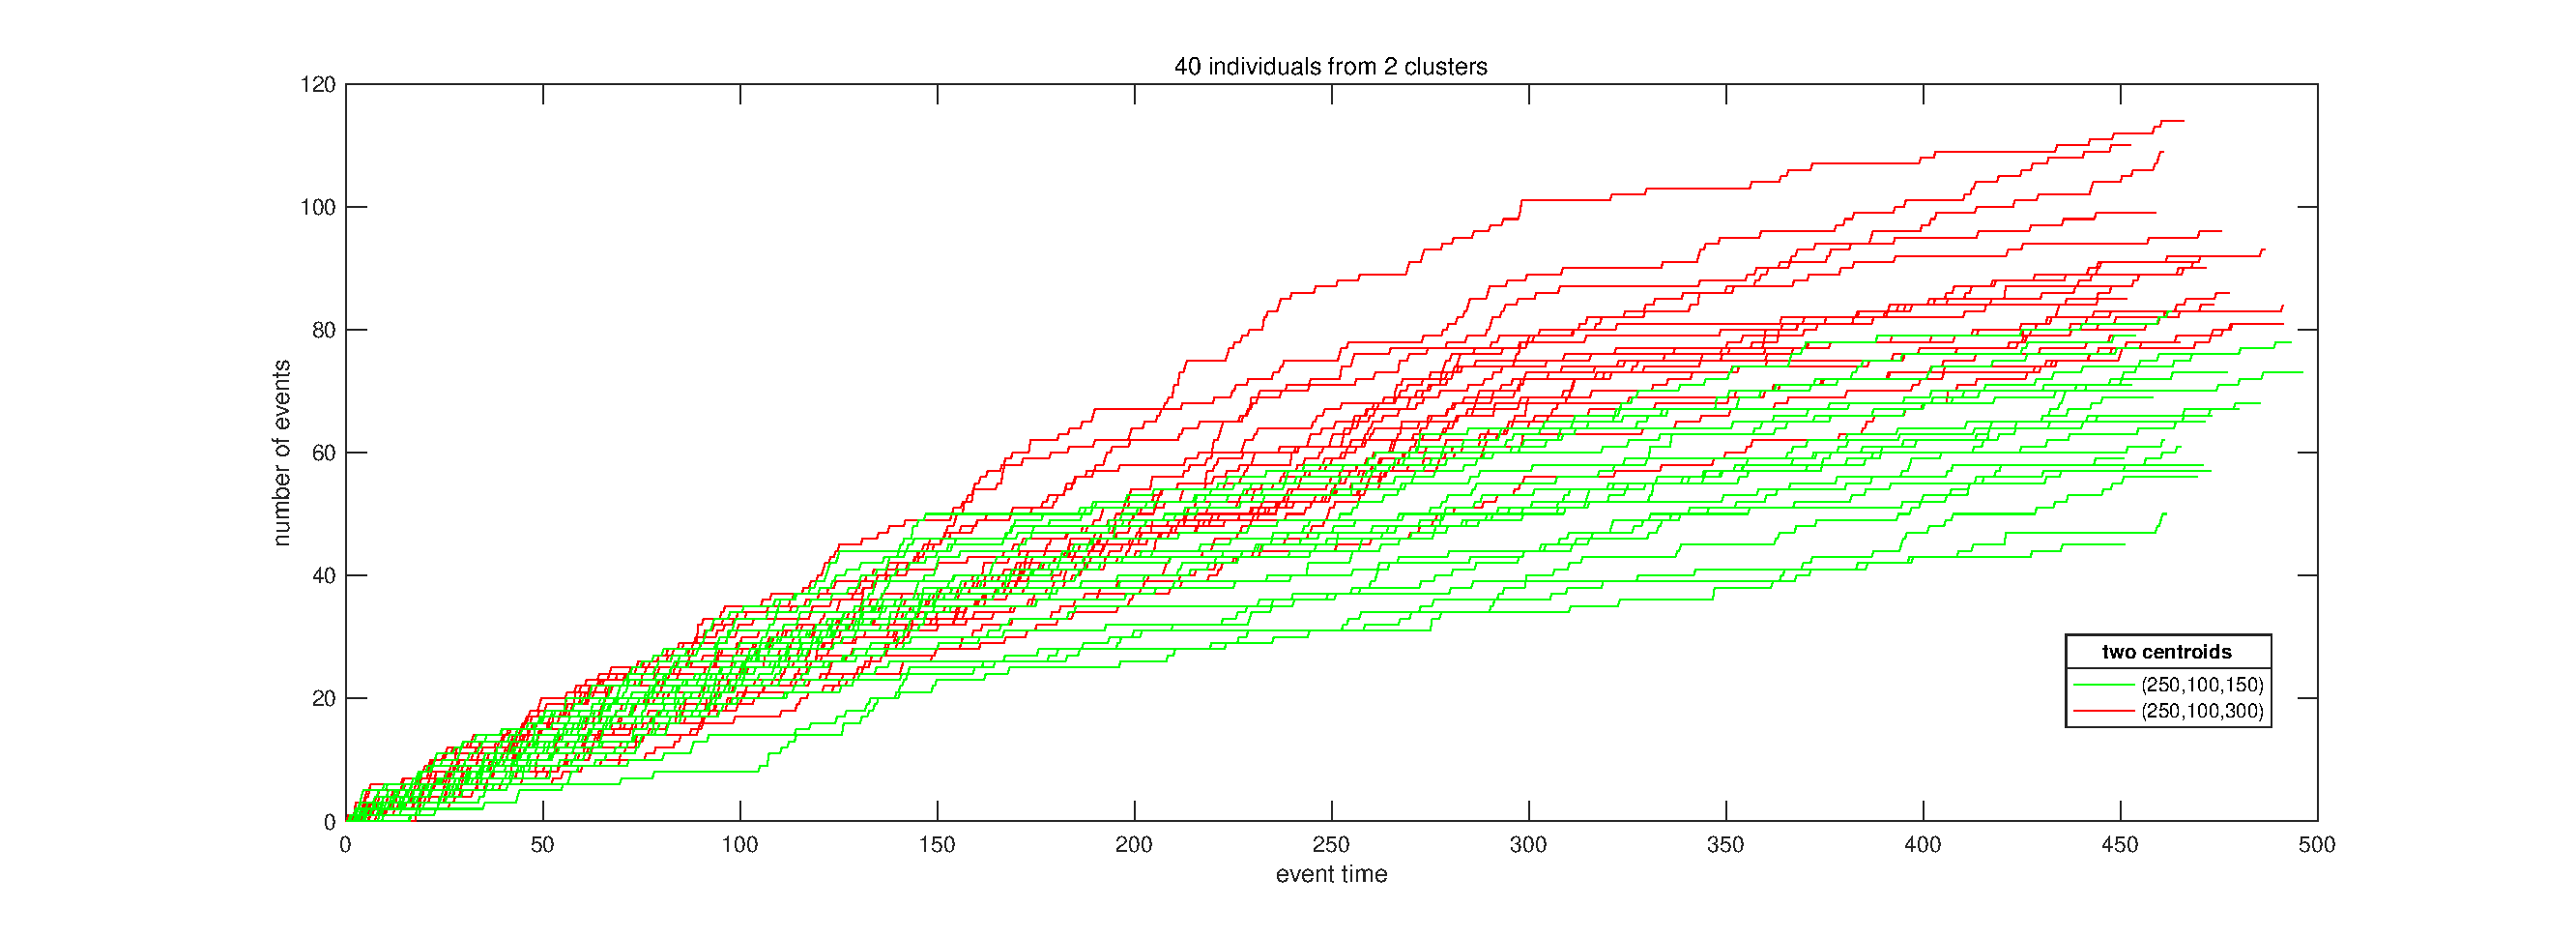
\includegraphics[width=\textwidth,height=0.6\textheight]{./figure/forty_lines.eps}
  \vspace{-30pt}
  \caption{40 lines from 2 clusters  }\label{fig:forty_lines}
  %\vspace{-10pt}
\end{figure} % truncate the kernal fitting





More formally, the natural thought of clustering individuals with recurrent events is clustering curves representing individuals. \citet{dass2015clustering} proposed a nonparametric Bayesian approach to cluster individuals with recurrent events. However, that approach mainly focused on finding the local change-point of different curves. If the change-point of two groups are the same, but the intensity rate functions are different, it could hardly divide them. Another method mentioned in \cite{perets2011clustering} is intuitive. The main idea of this method is extracting the characteritic of each time-to-event curve in \ref{fig:forty_lines}, then reduce the dimension of the data to a few principle components. However it is hard to achieve a good accuracy while implemented in recurrent event cases, because it loses the information that data are from a NHPP, which means the curves are non-decresing and piecewise constant.  

We propose a heuristic method, which is motivated by the k-means method. Unlike the k-means problem, which aimes to find cluster centers that minimize the intra-class variance, our method tries to find cluster centers which maximizes the likelihood of the underlying clusters given the observed data. To further illustrate the idea, suppose there are $K$ underlying groups, each group has one centroid, so there are K centroids in total. The purpose of the algorithm is to find the K underlying centroids and determine which individual belongs to which centroid. Denote $P_{jk}=P(\pmb X_j|\tau_k,\lambda_{kb},\lambda_{ka},c_j)$, which is the sampling density value given that individual $j$ falls in group $k$.
\begin{equation}\label{eqn:Pjk}
P_{jk}=exp[-\Lambda(c_j)]\prod_{i=1}^{n_j}\lambda_j(t_{ji})=exp[-\Uplambda(c_j)]\lambda_{kb}^{n_j^{(b)}}\lambda_{ka}^{n_j^{(a)}}
\end{equation}
The updating procedure for K centroids follow the same schema in \cite{hartigan1979algorithm}. Briefly, the first step is to initialize $K$ centroids. Next, for each individual $j$, assign it to the centroid $k^*$, where $k^*=argmax_{k=1,2,...K} P_{jk}$,then update the centroids of $K$ clusters using Eq.$(2)$ and Eq.$(3)$ until all the $K$ centroids finally do not change. We will illustrate the algorithms in detail as follows. And for notation convenience, we call our algorithm RKmeans in the following paper.

\begin{enumerate}[Step 1:]


\item set the initial value for the K centroids, denote as $(\lambda_{kb}^{(0)},\lambda_{ka}^{(0)},\tau_k^{(0)},k=1,...K)$. Like the original k-means problem, the estimation of the K centroids can be arbitrarily bad when the K initial centroids are poorly selected, with the extreme case when all K clusters are almost the same. So the intuition behind our initialization method is to spread out the K initial cluster centroids. One feasible solution is to use some careful random seeding method like k-means++ \ref{arthur2007k}, which improves both the speed and the accuracy of initialization. Now we will briefly introduce how it works in our dataset. 


\begin{enumerate}[(1):]
\item Select an individual $j$ with equal propability among all $m$ individuals. Then, as a special case with only one individual, calculate the centroids of the first cluster based on using the formula $2$,$3$ in \ref{sec:MLE}.
\item Denote $d_{jk}=|log(P_{jk})|$ as the distance from $j$ to cluster $k$.for each individual $j$, compute $d_{jk}$, the distance between $j$ and the nearest centroids that has been chosen.

\item choose one individual $j$ at random , using the weighted probability distribution where $j$ is chosen with probability proportional to $d_{jk}^2$, then calculate the centroids of the second cluster based on using the Eq.$(2)$ and Eq.$(3)$ in \ref{sec:MLE}.

\item Repeat Steps 2 and 3 until the $K$ centroids are chosen , so $\tau_{k}^{(1)},\lambda_{kb}^{(1)},\lambda_{ka}^{(1)},k=1,...K$ are the initial centroids.
\end{enumerate}



\item set $t=1$.
\item Under the condition that $K$ centroids $(\tau_{k}^{(t)},\lambda_{kb}^{(t)},\lambda_{ka}^{(t)}),k=1,...K$ are given, for each individual $j$,  assign $j$ to cluster $k$ which yields the largest sample density probability $P_{jk}$. After m calculations, all the individuals are assigned to $K$ clusters. For each cluster $k$, $G_k^{(t)}=\{j:P_{jk}>=P_{jk^{'}},\forall k^{'},1 \leq k^{'}\leq K,j\in\{1,...m\}\}$.

\item Update the centroids of cluster $k$ using Eq.$(2)$ and Eq. $(3)$

\begin{equation}\label{eqn:tau_MLE}
\hat{\tau_k}^{(t+1)}= argmax_{\tau_k = t_{ji}|j \in G_k^{(t)}, 1\leq i \leq n_j}logL_{(k)}(\tau_k,\hat\lambda_{kb},\hat\lambda_{ka}|\pmb X_{(k)}).
\end{equation}

\begin{equation}\label{eqn:lam_MLE}
\hat{\lambda}_{kb}^{(t+1)}=\frac{\sum_{j \in G_k^{(t)}}n_j^{(b)}}{\hat{\tau_k}^{(t+1)}N_k},\hat{\lambda}_{ka}^{(t+1)}=\frac{\sum_{j \in G_k^{(t)}}n_j^{(a)}}{\sum_{j \in G_k^{(t)}}c_j- \hat{\tau_k}^{(t+1)}N_k}.
\end{equation}

\item Repeat the assignment step and update step until $(\tau_{k}^{(t)},\lambda_{kb}^{(t)},\lambda_{ka}^{(t)})=(\tau_{k}^{(t+1)},\lambda_{kb}^{(t+1)},\lambda_{ka}^{(t+1)}),k=1,...K$. 
\item We use the $K$ centroids output by the last iteration as the estimator of our true cluster centroids.
\end{enumerate}



\subsection{Determine the number of clusters using a heuristic searching method}




In \ref{sec:kmean} , we suppose $m$ observations from $K$ centroids, where $K$ is given. However, in real datasets, $K$ is usually unknown. Though it can be determined using some empirical knowledge, we are more interested in finding a way to automatically determine the number of clusters based on the data. Fraley introduced some methods in \cite{fraley1998many}, to find the appropriate number of cluster $K$. One way is to use Bayesian Model Selection in clustering. The advantage of this method is that it uses the Bayes factor to compare different models. Because different $K$  different models, so determining the number of clusters is actually a model selection problem. Suppose the possible value for $K$ is only 1 or 2, and the observed data is $D$, the Bayes factor is assessed by $\frac{Pr(D|K=1)}{Pr(D|K=2}=\frac{Pr(K=1|D)}{Pr(K=1|D)}\frac{Pr(K=2)}{Pr(K=1)}$. The advantage of this Bayes factor is that it naturally includes a penalty term $\frac{Pr(K=2)}{Pr(K=1)}$. But it is really hard to figure out how to set the prior of $Pr(K)$ to avoid choosing a large $K$, since $Pr(D|K)$ is always an incresing function as K becomes larger. Another way is to use Akaike information criterion mentioned in \cite{akaike1998information} to qualify the model. Here, we can use $AIC=2p-2ln(\hat{L})$, where $p$ is the number of estimated parameters in the model. $\hat{L}$ is the maximum value of the likelihood function for the model. Pick the model with the smallest $AIC$ value. However, when using this criteria in calculation, the second term $ln(\hat(L))$ is often much larger than the first penalty term $2p$, meaning that the $AIC$ value is dominated by $ln(\hat{L})$, thus using $AIC$ criteria to choose the appropriate $K$ is not a good option.



We use a heurastic searching method, combining the idea of large sample inference and non-parametric hypothesis testing. The method can be divided into two parts,testing part and searching part. First we will go through the testing part and establish the required notations. Denote $\pmb q_{(K)}=(\pmb q_1,\cdots,\pmb q_K)^T$, where $\pmb q_k=(\tau_k,\lambda_{kb},\lambda_{ka})^T$ as the centroid of $k^{th}$ group. Then define $\pmb X_{\pmb q_{(K)}}=(\pmb X_1,...\pmb X_m)$ as the random dataset generated from $\pmb q_{(K)}$.  Suppose we use RKmeans in \ref{sec:kmean} to cluster $\pmb X_{\pmb q_{(K)}}$ into $n$ groups, then:
\begin{enumerate}[(1):]
\item Denote $\hat{\pmb q_{(n)}}(\pmb X)$ as the estimate of $n$ centroids using RKmeans based on data $\pmb X$. Hence write  $\hat{\pmb q_{(n)}}(\pmb X_{\pmb q_{(n)}})=(\hat{\pmb q_1},\cdots,\hat{\pmb q_{n}})$ as the estimate of $n$ centroids based on data $\pmb X_{\pmb q_{(K)}}$.

\item Denote $p_{\pmb q_{(n)}}(\pmb X)=\prod_{i=1}^{n}\prod_{j\in G_i}P_{ji} $ as the sample probability density value while assuming data $X$ are generated from $\pmb q_{(n)}$. Here, $G_i,i=1,\cdots,n$ can be calculated using RKmeans based on the data $\pmb X$ and the estimated centroids $\hat{\pmb q_{(n)}}(\pmb X)$. Thus $p_{\hat{\pmb q_{(n)}}}(\pmb X_{\pmb q_{(K)}})=\prod_{i=1}^{n}\prod_{j\in G_i}P_{ji} $, which is the sample probability density value while  $\pmb X_{\pmb q_{(K)}}$ are generated from its estimated centroids $\hat{\pmb q_{(n)}}(\pmb X_{\pmb q{(K)}})$.
  
\item Denote $Y_{(n)}(\pmb X)=log \frac{p_{\hat{\pmb q_{(n+1)}}}(\pmb X)}{p_{\hat{\pmb q_{(n)}}}(\pmb X)}$  as the log ratio of probabililty that $X$ are generated from $\hat{\pmb q_{(n+1)}}(\pmb X)$ divided by the probability that $X$ are generated from $\hat{\pmb q_{(n)}}(\pmb X)$. Thus, $Y_{(n)}(\pmb X_{\pmb q_{(K)}})=log \frac{p_{\hat{\pmb q_{(n)}}}(\pmb X_{\pmb q_{(K)}})}{p_{\hat{\pmb q_{(n)}}}(\pmb X_{\pmb q_{(K)}})}$ is the log ratio of  $p_{\hat{q_{(n+1)}}}(\pmb X_{\pmb q_{(K)}})$ divided by  $p_{\hat{q_{(n)}}}(\pmb X_{\pmb q_{(K)}})$.

\end{enumerate}

The intuition behind is straight-forward. Suppose the real data $\pmb X^*$ has $K^*$ underlying groups, denoted as $\pmb q_{(K^*)}^*$. When we do not know the true value of $K_1$, we usually suggest the data coming from $K$ groups, then test whether $K$ is appropriate. To construct the test, first, estimate the centroids of $K$ groups based on $\pmb X^*$, which is $\hat{\pmb q_{(K)}}(X^*)$.  We can assume the real data is a random sample of $\pmb X_{\hat{\pmb q_{(K)}}}$. If $K=K^*$, the real data is also a random sample of $\pmb X_{q_{(K^*)}}$. Under $K=K^*$, let $\pmb q_{(K^*)}^*= \hat{\pmb q_{(K)}}(X^*)$, and generate $B$ datasets based on $\pmb q_{(K^*)}^*$, denoted as $\pmb X_{\pmb q_{(K^*)}^*}^{(1)},\cdots,\pmb X_{\pmb q_{(K^*)}^*}^{(B)}$. Calculate $Y_{(K)}(\pmb X_{\pmb q_{(K^*)}^*}^{(i)}),i=1,\cdots,B$ on each smaple data, we get $B$ samples from random variable $Y_{(K)}(\pmb X_{\pmb q_{(K^*)}^*})$. Also calculate $Y_{(K)}(\pmb X^*)$ based on the real data $\pmb X^*$. Because $\pmb X^*$ can also be considered as a sample of $\pmb X_{\pmb q^*_{(K^*)}}$. Intuitively, if the data is actually generated from $K$ clusters, $Y_{(K)}(\pmb X^*)$ should be as similar as $Y_{(K)}(\pmb X_{\pmb q_{(K^*)}^*}^{(i)}),i=1,\cdots,B$, which means  $Y_{(K)}(\pmb X^*)$ should not be larger or smaller than most of the  $Y_{(K)}(\pmb X_{\pmb q_{(K^*)}^*}^{(i)})$. Thus, if $Y_{(K)}(\pmb X^*) \geq Y_{(K)}(\pmb X_{\pmb q_{(K^*)}^*}^{(i)}),\forall i=1,\cdots,B$, we don't think $Y_{(K)}(\pmb X^*)$ is a sample of $Y_{(K)}(\pmb X_{\pmb q_{(K^*)}^*})$. So if the strong evidence shows that $Y_{(K)}(\pmb X^*)$ has a low chance being a sample of $Y_{(K)}(\pmb X_{\pmb q_{(K^*)}^*})$, we reject the hypothesis that $K^*=K$. To derive a more formal way to construct the test, we introduce two methods to test whether $Y_{(K)}(\pmb X^*)$ can be considered as a sample from $Y_{(K)}(\pmb X_{\pmb q_{(K^*)}^*})$ or not. First method is simple and computational efficient, second method is a little complicated but more robust to the outliers.


\begin {enumerate}[Method 1:]
\item Denote $T_1=\Sigma_{i=1}^B \pmb 1(Y_{(K)}(\pmb X^*) \geq Y_{(K)}(\pmb X_{\pmb q_{(K^*)}^*}^{(i)}))$,$T_1=\Sigma_{i=1}^B \pmb 1(Y_{(K)}(\pmb X^*) \leq Y_{(K)}(\pmb X_{\pmb q_{(K^*)}^*}^{(i)}))$ where $\pmb 1(.)$ is the indicator function. Let $T=\frac{max\{T_1,T_2\}}{B}$, when $T$ is close to $1$, it means either  $\pmb Y_{(K)}(\pmb X^*)$ is greater or smaller than most of  $Y_{(K)}(\pmb X_{\pmb q_{(K^*)}^*}^{(i)}),i=1,\cdots,B$, which can be considered as the extreme case if we assume they are from the same distribution. Usually,for simplicity, when we observe $T \geq 0.95$, we reject  $K_1=K$.

\item Another way is to use resampling method on the original data $\pmb X^*$ to get new datasets similar as $\pmb X^*$, the basic idea is motivated by bootstraping \cite{efron1994introduction}, which is by resampling the sample data and performing inference about a sample from resampled data. The procedure of resampling $\pmb X^*$ is just sampling from its elements $(\pmb X_1^*,\cdots,\pmb X_m^*)$ with equal probability and rearrange them from $1,\cdots,m$. Suppose we resample $B$ times based on $\pmb X^*$, the $i^{th}$ resampled data can be written as  $\pmb X^{*^{(i)}}=(\pmb X_1^{*^{(i)}},\cdots,\pmb X_m^{*^{(i)}}),i=1,\cdots,B$, where $\pmb X_j^{*^{(i)}} \in \pmb X^*,\forall j \in \{1,\cdots,m\}$. After we get the resampled data, we can compute $Y_{(K)}(\pmb X^{*^{(i)}}),i=1,\cdots,B$ as the resampled data from $Y_{(K)}(\pmb X^*)$. Now we have two sequence of samples, one is $Y_{(K)}(\pmb X_{\pmb q_{(K^*)}^*}^{(i)}),i=1,\cdots,B$, which are $B$ random samples of $Y_{(K)}(\pmb X_{\pmb q_{(K^*)}^*})$, the other is  $Y_{(K)}(\pmb X^{*^{(i)}}),i=1,\cdots,B$ , which are $B$ bootstrap samples of $Y_{(K)}(X^*)$. If $K^*=K$, the two sequence of samples should be as similar as each other. Here, we use Wilcoxon rank-sum test \cite{wilcoxon1945individual}, which is a non-parametric statistical hypothesis test used to compare two independent samples to assess whether they are from the population with the same distribution or not. If the test rejects that they are from the same distribution, the assumption that $K_1=K$ is also rejected.
  
\end {enumerate} 

Note: 
\begin{enumerate}[(1):]
\item Usually, we set $B=1000$ to guarantee the sample size is large enough for measuring the properties of the random variable $Y_{(K)}(\pmb X)$.
\item In simulation study, when $K<K^*$, $Y_{(K)}(\pmb X^*)$ is usually much larger than the samples of $Y_{(K)}(\pmb X_{\pmb q_{(K^*)}^*})^{(i)},i=1,\cdots,B$ . For example, suppose our data are generated from two groups with centroids $(250,100,300)$ and $(250,100,150)$ respectively, thus $K^*=2$. When $K=1<K^*$, perform the test procedure, and the plot \ref{fig:sample_distribution} shows the sample distribution of $Y_{(K)}(\pmb X_{\hat{\pmb q_{(1)}}(\pmb X^*)})$ and the bootstrap samples of $Y_{(K)}(\pmb X^*)$. Based on Wilcoxon rank-sum test, the assumption that $K^*=1$ is rejected.

\item The second method performs slightly better than the alternative one.

\end{enumerate}

\begin{figure} [htp]
 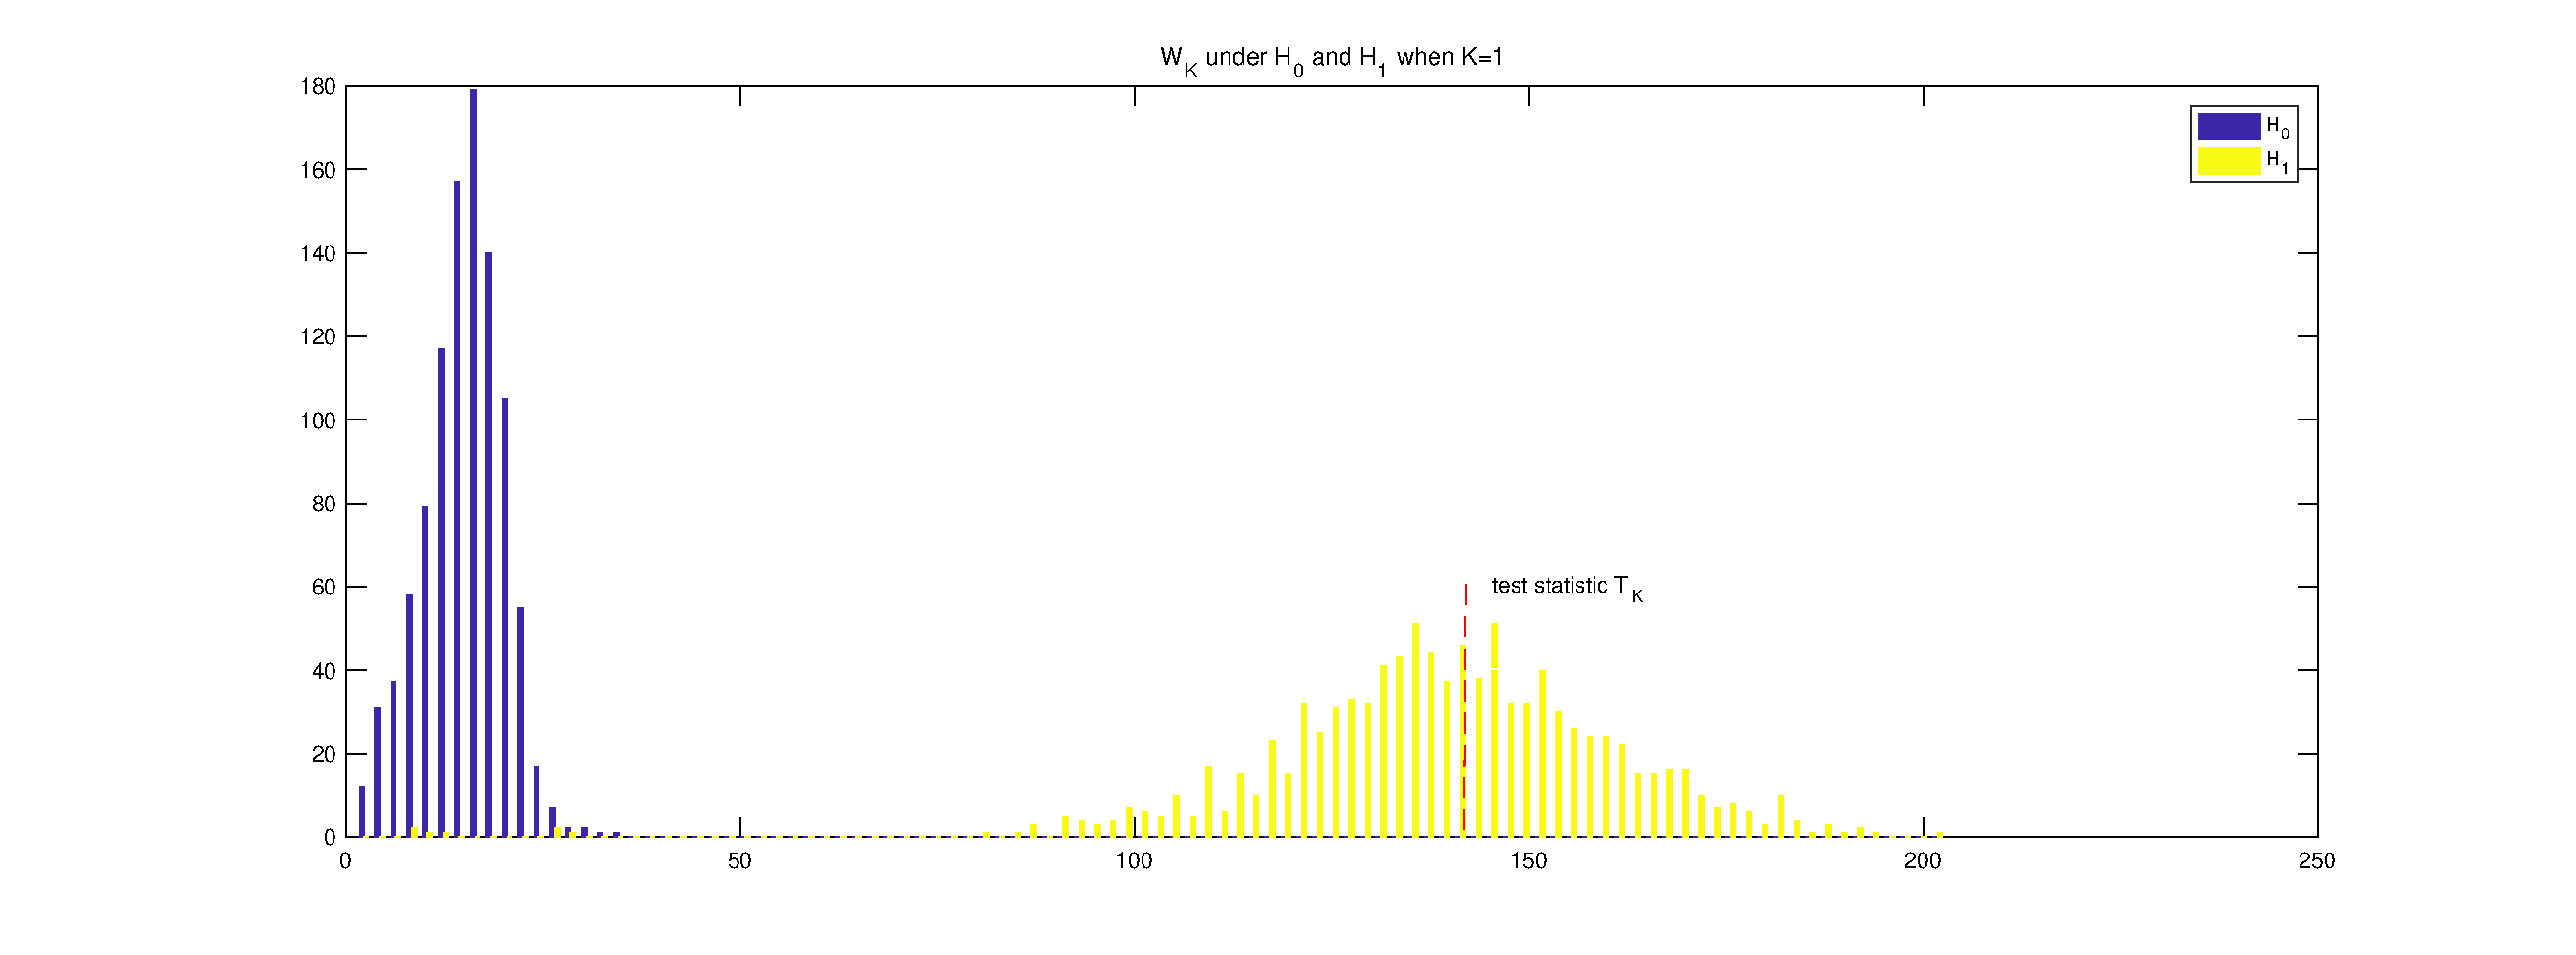
\includegraphics[width=\textwidth,height=0.6\textheight]{./figure/sample_distribution.eps}
  \vspace{-30pt}
  \caption{sample distribution }\label{fig:sample_distribution}
  %\vspace{-10pt}
\end{figure} % truncate the kernal fitting


After deriving a method to assess whether $K$ clusters is appropriate for the observed data $X^*$. We can start searching the appropriate number of clusters iteratively, basically start from $K=1$ and end searching when we have found the smallest $K$ that satisfy the retaining condition of the test procedure.

Finally,we write the compact solution to determine the number of clusters as follows.


\begin{enumerate}[Step 1:]
  
\item Starting from K=1.
\item Testing $K^*=K$ using Method 1 or Method 2 in the testing procedure mentioned above, if the test rejects $K^*=K$, reset $K=K+1$. Otherwise, accept the assumption that $K^*=K$.

  
\end{enumerate}

Note:
  Notice that the test procedure is conservative. For example, if the assuption that $K=2$ is not rejected, we will conclude that data are generated from two groups and will not test whether it is possible that the data are generated from $K \geq 2$ clusters.







\section{Simulation Studies}\label{sec:simulation}
We run simulations to check the performance of the methodology proposed in Section \ref{sec:models.kmean} in different scenarios. Data is generated from a NHPP with piecewise-constant intensity functions according to the distribution of the inter-event times \citep{Klein1984}. The data in simulation is generated as follows. Given the ordered time to events $T_0=t_0=0, ~T_1=t_1, ~\cdots, ~T_{i}=t_{i}$, the cumulative density function (CDF) of the $(i+1)^{th}$ inter-event time $X_{i+1}=T_{i+1}-T_{i}$ for each individual is: 
\begin{equation}\label{eqn:Ft}
\begin{aligned}
 F_{i+1}(x)&=Pr\left[ X_{i+1}\leq x|T_p=t_p,~p=1,2, \cdots, i\right] \\
&=1-exp\left[ \varLambda(t_{i})-\varLambda(t_{i}+x)\right],
\end{aligned}
\end{equation}
where  $\varLambda(\cdot)$ is the cumulative intensity function of the NHPP. Then $t_{i+1}=x_{i+1}+t_i$. 

Starting from $i=0$, the detailed algorithm is: 
\begin{enumerate}[Step 1:]
  \item Sample $x_{i+1}$ from a distribution with CDF $F_{i+1}$;
  \item $t_{i+1}=t_{i}+x_{i+1}$;
  \item $i=i+1$, return to Step (1).
\end{enumerate} 
The above process is run until $t_{i+1}$ is larger than the censoring time $C_j$. $t_1, ~t_2,~ \cdots, ~t_i$ are the ordered times to event for the $j^{th}$ subject. 

\subsection{Simulation settings}
Tables \ref{tab:setd} are the eleven setting with configurations of different change-points, intensity rates, mixing proportions, number of clusters.

\begin{table}[htp]
  \caption{\label{tab:setd}Nine settings for the simulation}
    \vspace{1ex}
 \centering
 \begin{tabular}{cl}
\hline
Setting&\multicolumn{1}{p{14.5cm}}{Description }\\ \hline
1 & \multicolumn{1}{p{14.5cm}}{The number of subjects are $m=40$. The sample unit has the same probability generated from two clusters with centroids equal to $(\mu_1=150,\lambda_{1b}=250,\lambda_{1a}=100)$ and $(\mu_2=300,\lambda_{1b}=250,\lambda_{1a}=100)$ respectively.}\\

2& \multicolumn{1}{p{14.5cm}}{Identical as Setting 1 except for the number of subjects becomes $m=80$, thus $N_1 = N_2 = 40$. }\\

3& \multicolumn{1}{p{14.5cm}}{Identical as Setting 1 except for the centroid of the second cluster is different, which is  $(\mu_2=200,\lambda_{2b}=250,\lambda_{2a}=100)$}\\

4& \multicolumn{1}{p{14.5cm}}{Identical as Setting 1 except for the centroids of two clusters become $(150,250,200)$ and $(300,250,200)$ respectively}\\

5& \multicolumn{1}{p{14.5cm}}{Identical as Setting 1  except for unbalanced clusters' sizes, for example, $N_1 = 30, N_2 = 10$}\\

6& \multicolumn{1}{p{14.5cm}}{Identical as Setting 1  except for the censoring time for each sample unit $ \sim (10, 500)$}\\

7& \multicolumn{1}{p{14.5cm}}{Identical as Setting 1  except for the change-points of each cluster has a variation of $Unif(-5, 5)$, where $\mu_1 \sim Unif(245, 255)$ and $\mu_2 \sim Unif(95, 105)$}\\

8& \multicolumn{1}{p{14.5cm}}{Identical as Setting 1  except for the intensity rates are generated from gamma distribution.  $\lambda_{1b},\lambda_{2b} \sim Gamma(25, 100)$, $\lambda_{1a},\lambda_{2a}\sim Gamma(10, 100)$ }\\

9& \multicolumn{1}{p{14.5cm}}{Identical as Setting 1  except for the centroids of two clusters become $(150,250,100)$ and $(300,100,250)$}\\

10& \multicolumn{1}{p{14.5cm}}{Identical as Setting 1  except for the centroids of two clusters become $(150,250,100)$ and $(150,100,250)$}\\
   
11& \multicolumn{1}{p{14.5cm}}{The number of subjects are $m=40$. The sample unit has the same probability generated from three clusters with centroids equal to $(\mu_1=100,\lambda_{1b}=250,\lambda_{1a}=100)$ ,$(\mu_2=200,\lambda_{1b}=200,\lambda_{1a}=100)$ and $(\mu_3=300,\lambda_{1b}=250,\lambda_{1a}=100)$ respectively.}\\

12& \multicolumn{1}{p{14.5cm}}{The number of subjects are $m=40$. The sample unit has the same probability generated from four clusters with centroids equal to $(\mu_1=100,\lambda_{1b}=250,\lambda_{1a}=100)$ ,$(\mu_2=150,\lambda_{1b}=150,\lambda_{1a}=100)$, $(\mu_3=200,\lambda_{1b}=250,\lambda_{1a}=100)$ and $(\mu_4=250,\lambda_{1b}=250,\lambda_{1a}=100)$ respectively.}\\\hline
  

    \end{tabular}%
\end{table}%
\subsection{Simulation Results}


   \begin{table}[htp]
  %\vspace{-30pt} 
   \caption{\label{tab:set1}Simulation results of  Settings 1-5.}
     \vspace{1ex}
  \centering
  \begin{tabular}{cccrS[table-format=2.2]S[table-format=2.2]c}
  \hline\hline
 Setting
 &Parameter
 &\multicolumn{1}{p{1.2cm}}{\centering True value}
 &\multicolumn{1}{p{1.4cm}}{\centering Average of\\ estimates}
 &\multicolumn{1}{c}{RMSE}
 & \multicolumn{1}{c}{$|$Bias (\%)$|$}
 &\multicolumn{1}{p{2.0cm}}{\centering Coverage probability (\%)} \\ \hline
 \multirow{5}{*}{1}&$\mu_1$         & 150   & 149.01  & 2.23  & 0.66  & 95.0  \\
&$\mu_2$  & 300   & 300.08  & 1.31  & 0.03  & 90.0   \\
&$\lambda_{1b}$  & 250   & 249.9   & 0.01  & 0.04  & 97.5       \\
&$\lambda_{2b}$       & 250   & 252.87  & 0.01  & 1.15  & 95.0       \\
&$\lambda_{1a}$  & 100   & 100.18  & 0.00  & 0.18  & 92.5       \\
&$\lambda_{2a}$  & 100   & 99.59   & 0.01  & 0.41  & 97.5      \\ \hline

\multirow{5}{*}{2}
&$\mu_1$         & 150   & 149.78  & 0.81  & 0.14  & 90.0   \\
&$\mu_2$  & 300   & 299.98  & 1.00  & 0.01  & 92.5   \\
&$\lambda_{1b}$  & 250   & 253.01  & 0.01  & 1.20  & 77.5      \\
&$\lambda_{2b}$  & 250   & 249.56  & 0.01  & 0.17  & 90.0       \\
&$\lambda_{1a}$  & 100   & 99.78   & 0.00  & 0.22  & 92.5     \\
&$\lambda_{2a}$  & 100   & 99.45   & 0.00  & 0.55  & 92.5     \\\hline

\multirow{5}{*}{3}
&$\mu_1$         & 150   & 149.10  & 2.39  & 0.60  & 97.5   \\
&$\mu_2$  & 200   & 199.45  & 2.81  & 0.28  & 97.5  \\
&$\lambda_{1b}$  & 250   & 250.92  & 0.01  & 0.37  & 95.0      \\
&$\lambda_{2b}$  & 250   & 253.51  & 0.01  & 1.40  & 95.0       \\
&$\lambda_{1a}$  & 100   & 97.56   & 0.01  & 2.44  & 97.5     \\
&$\lambda_{2a}$  & 100   & 100.97  & 0.01  & 0.97  & 100.0     \\\hline

\multirow{5}{*}{4}
&$\mu_1$         & 150   & 149.18  & 1.56  & 0.55  & 85.0    \\
&$\mu_2$  & 300   & 299.84  & 1.41  & 0.05  & 85.0   \\
&$\lambda_{1b}$  & 250   & 249.87  & 0.01  & 0.05  & 92.5    \\
&$\lambda_{2b}$  & 250   & 249.18  & 0.01  & 0.33  & 90.0      \\
&$\lambda_{1a}$  & 100   & 99.55   & 0.00  & 0.45  & 90.0     \\
&$\lambda_{2a}$  & 100   & 100.16  & 0.00  & 0.16  & 85.0       \\\hline

\multirow{5}{*}{5}
&$\mu_1$         & 150   & 150.17  & 3.73  & 0.11  & 100.0   \\
&$\mu_2$  & 300   & 300.51  & 1.25  & 0.17  & 95.0   \\
&$\lambda_{1b}$  & 250   & 247.16  & 0.01  & 1.13  & 100.0     \\
&$\lambda_{2b}$  & 250   & 250.4   & 0.01  & 0.16  & 100.0      \\
&$\lambda_{1a}$  & 100   & 99.74   & 0.01  & 0.26  & 97.5    \\
&$\lambda_{2a}$  & 100   & 100.64  & 0.00  & 0.64  & 87.5      \\\hline


\hline
     \end{tabular}%
 \end{table}%


    \begin{table}[htp]
  %\vspace{-30pt}
   \caption{\label{tab:set1}Simulation results for Settings 6-10. }
     \vspace{1ex}
  \centering
  \begin{tabular}{cccrS[table-format=2.2]S[table-format=2.2]c}
  \hline\hline
 Setting
 &Parameter
 &\multicolumn{1}{p{1.2cm}}{\centering True value}
 &\multicolumn{1}{p{1.4cm}}{\centering Average of\\ estimates}
 &\multicolumn{1}{c}{RMSE}
 & \multicolumn{1}{c}{$|$Bias (\%)$|$}
 &\multicolumn{1}{p{2.0cm}}{\centering Coverage probability (\%)} \\ \hline

\multirow{5}{*}{6}
&$\mu_1$         & 150   & 149.90  & 2.88  & 0.06  & 87.5   \\
&$\mu_2$  & 300   & 299.55  & 1.05  & 0.15  & 77.5  \\
&$\lambda_{1b}$  & 250   & 250.46  & 0.01  & 0.18  & 92.5      \\
&$\lambda_{2b}$  & 250   & 251.12  & 0.01  & 0.45  & 97.5     \\
&$\lambda_{1a}$  & 100   & 98.29   & 0.00  & 1.71  & 100.0     \\
&$\lambda_{2a}$  & 100   & 101.8   & 0.01  & 1.80  & 95.0      \\\hline

\multirow{5}{*}{7}
&$\mu_1$         & 150   & 151.05  & 2.07  & 0.70  & 97.5   \\
&$\mu_2$ & 300   & 300.64  & 2.72  & 0.21  & 87.5  \\
&$\lambda_{1b}$  & 250   & 246.90  & 0.01  & 1.24  & 90.0      \\
&$\lambda_{2b}$  & 250   & 247.99  & 0.01  & 0.80  & 90.0     \\
&$\lambda_{1a}$  & 100   & 100.79  & 0.00  & 0.79  & 87.5     \\
&$\lambda_{2a}$  & 100   & 102.21  & 0.00  & 2.21  & 97.5\\\hline

\multirow{5}{*}{8}
&$\mu_1$         & 150   & 148.81  &2.39	&0.79	&100.0\\
&$\mu_2$  & 300   & 298.76	&2.32	&0.41	&92.5\\
&$\lambda_{1b}$  & 250   & 249.61	&0.01	&0.16	&92.5  \\
&$\lambda_{2b}$  & 250   & 248.46	&0.01	&0.62	&95\\
&$\lambda_{1a}$  & 100   & 93.89	&0.01	&6.11	&97.5    \\
&$\lambda_{2a}$  & 100   & 101.99   & 0.01  & 1.99 & 95.0      \\\hline

\multirow{5}{*}{9}
&$\mu_1$         & 150   & 150.1	&2.27	&0.07	&97.5	 \\
&$\mu_2$  & 300   &300.16	&1.34	&0.05	&90	\\
&$\lambda_{1b}$  & 250   & 253.56	&0.01	&1.42	&77.5 \\
&$\lambda_{2b}$  & 100   & 101.59	&0.15	&1.59	&85\\
&$\lambda_{1a}$  & 100   & 101.74	&0.01	&1.74	&87.5 \\
&$\lambda_{2a}$  & 250   & 248.31	&0.15	&0.67	&92.5   \\\hline

\multirow{5}{*}{10}
&$\mu_1$         & 150   & 150.8	&1.89	&0.53	&90.0	 \\
&$\mu_2$         & 150   & 150.22	&0.95	&0.15	&85.0	\\
&$\lambda_{1b}$  & 100   & 99.68	&0.00	&0.32	&95.0 \\
&$\lambda_{2b}$  & 250   & 246.96	&0.01	&1.22	&95.0\\
&$\lambda_{1a}$  & 250   & 248.38	&0.01	&0.65	&95.0 \\
&$\lambda_{2a}$  & 100   & 99.89	&0.00	&0.11	&95.0   \\\hline
\hline
     \end{tabular}%
 \end{table}%


    \begin{table}[htp]
  %\vspace{-30pt}
   \caption{\label{tab:set1} Simulation results for Settings 11-12}
     \vspace{1ex}
  \centering
  \begin{tabular}{cccrS[table-format=2.2]S[table-format=2.2]c}
  \hline\hline
 Setting
 &Parameter
 &\multicolumn{1}{p{1.2cm}}{\centering True value}
 &\multicolumn{1}{p{1.4cm}}{\centering Average of\\ estimates}
 &\multicolumn{1}{c}{RMSE}
 & \multicolumn{1}{c}{$|$Bias (\%)$|$}
    &\multicolumn{1}{p{2.0cm}}{\centering Coverage probability (\%)} \\ \hline

\multirow{2}{*}{11}
&$\mu_1$         & 100   & 99.92	&0.73	&0.08	&100.0	 \\
&$\mu_2$         & 200   & 200.86	&2.57	&0.43	&100.0	\\
&$\mu_3$  & 300   & 299.58	&2.06	&0.14	&97.5 \\
&$\lambda_{1b}$  & 250   & 255.30	&0.01	&2.12	&97.5\\
&$\lambda_{2b}$  & 250   & 246.81	&0.01	&1.27	&97.5 \\
&$\lambda_{3b}$  & 250   & 248.87	&0.01	&0.45	&100.0   \\
&$\lambda_{1a}$  & 100   & 100.08	&0.01	&0.08	&100.0\\
&$\lambda_{2a}$  & 100   & 97.80	&0.01	&2.20	&100.0 \\
&$\lambda_{3a}$  & 100   & 102.51	&0.01	&2.51	&97.5   \\\hline
    


\multirow{2}{*}{12}
&$\mu_1$         & 100   & 95.24	&13.76	&4.76	&100.0	 \\
&$\mu_2$         & 150   & 144.35	&25.14	&3.77	&100.0	\\
&$\mu_3$  & 200   & 204.03	&32.46	&2.01	&100.0 \\
&$\mu_4$  & 250   & 247.05	&18.61	&1.18	&100.0\\
&$\lambda_{1b}$  & 250   & 257.89	&0.03	&3.16	&100.0 \\
&$\lambda_{2b}$  & 250   & 260.05	&0.03	&4.02	&100.0   \\
&$\lambda_{3b}$         & 250   & 250.16	&0.02	&0.06	&100.0	 \\
&$\lambda_{4b}$         & 250   & 243.33	&0.02	&2.67	&100.0	\\
&$\lambda_{1a}$  & 100   & 99.27 	&0.01	&0.73	&100.0 \\
&$\lambda_{2a}$  & 100   & 97.98 	&0.01	&2.02	&100.0\\
&$\lambda_{3a}$  & 100   & 94.67	&0.01	&5.33	&100.0 \\
&$\lambda_{4a}$  & 100   & 102.41	&0.01	&2.41	&97.5   \\\hline    
\hline
     \end{tabular}%
 \end{table}%

 \begin{table}[htp]
  %\vspace{-30pt}
   \caption{\label{tab:set1}Two percentages for all the simulation settings, Note: $c_1$ is correctly estimated number of clusters(\%),$c_2$ is average percentage of correctly grouped subjects }
     \vspace{1ex}
  \centering
   \begin{tabular}{ccccccccccccc}
  \hline\hline
 \multicolumn{1}{p{1.2cm}}{Setting}
 &\multicolumn{1}{c}{ }
 &\multicolumn{1}{c}{$2$ } 
    &\multicolumn{1}{c}{$3$ }
       &\multicolumn{1}{c}{$4$ } 
    &\multicolumn{1}{c}{$5$ }
     &\multicolumn{1}{c}{$6$ }

       
    &\multicolumn{1}{c}{$7$ }
    &\multicolumn{1}{c}{$8$ }
    &\multicolumn{1}{c}{$9$ }
    &\multicolumn{1}{c}{$10$ }
    &\multicolumn{1}{c}{$11$ }
    &\multicolumn{1}{c}{$12$ }\\
    \hline
    $c_1$&97.5&97.5&80.00&97.05&92.50&100&97.50&85.0&97.5&100&77.5&90\\
    \hline
    $c_2$&98.65&98.65&88.05&98.21&97.77&99.50&99.10&92.35&99.10&100&75&77.31\\

    
\hline
     \end{tabular}%
 \end{table}%










\section{Conclusion and Discussion}\label{sec:discussion}
Based on the idea of \cite{perets2011clustering} and the assumption of our data, it's appropriate to represent each individual $j$ by a three dimension parameter set $\tau_j,\lambda_{jb},\lambda_{ja}$, which includes most of the information from the original data. The three dimension data can be viewed as a position in $R^3$ space, so we get m points in $R^3$
\section{Appendix}

\subsection{Data Generation}\label{sec:datageneration}

\bibliographystyle{apalike}
\bibliography{paper_kmean}
\end{document}

